A mitigation against many KASLR derandomization attacks is called \textit{Kernel Page Table Isolation} (\textit{KPTI}).
The concept was initially introduced under the name KAISER (\textit{Kernel Address Isolation to have Side-channels Efficiently Removed}) by D. Gruss et al.\cite{kaiser}.
Originally \textit{KAISER} was implemented as a patch for the Linux kernel and demonstrated on Ubuntu 16.10.
It was later adapted by the Linux kernel developers and merged into the mainline kernel (4.15) under the name KPTI.\cite{kpti_lwn}

\subsection{Problem}

The main cause for many KASLR derandomization attacks is improper information leakage after an illegal operation was performed or attempted to be performed by the CPU and not properly rolled back (i.e. caches not being cleared correctly, or timing differences in exception handling, page table traversals and memory accesses).
What all of these attacks rely on is that this initial information is accessed by the CPU and not properly guarded.
If this initial code path leading to the access could be avoided almost all attacks would be rendered unfunctional. \cite{kaiser}

In this case that would mean not mapping the kernel address space into userspace at all and vice-versa, which has been proposed by multiple papers before\cite{drk, prefetch-side-channel-smap}.

This is a very drastic and brute-force measure which would impact many things such as multithreaded applications or even contexts switches in general making some use cases practically impossible.
Multithreaded applications share the same address space per thread and thus switching to the kernel-only address space would break parallel execution of threads as the user address space would not be accessible anymore.
This would also incur a lot of TLB flushes as the address space would have to be completely switched with every syscall.\cite{kaiser}

Thus a less intrusive approach is needed.

\subsection{Challenges to overcome}

\textit{D. Gruss et al.} \cite{kaiser} identify three major challenges that have to be overcome or accomodated for in order for a solution to be viable.

\begin{itemize}
  \item{
    \textbf{Multithreading}:
    Threads share the same address space.
    Thus when a thread enters kernel mode and switches to a kernel-exclusive address space all other threads would switch to the same address space as well, partially defeating the original goal of the mitigation.
    A context switch would also mean having to synchronize all threads.
  }
  \item{
    \textbf{Implicitely assumed and required mappings}:
    Assumptions about the presence of user space mappings being present when in kernel mode and vice-versa are made in many places in the Linux kernel.
    These assumptions are often implicit and not easy to spot.
    The architecture of x86 processors requires that a few mappings are present at all times (i.e., when in user space and when in kernel space).
    Changes would have to be made to the kernel at large to accomodate for this, requiring a significant chunk of work.
  }
  \item{
    \textbf{Amount and impact of TLB flushes}:
    Switching the address space incurs an implicit full TLB flush and modifying the address space causes a partial TLB flush. \cite{the-ginormous-intel-manual-volume-3}
  }
\end{itemize}

\subsection{Approach}

The solution to the given problem by \textit{KAISER} deals with the above challenges.

Split the address space into two parts. First the \textit{shadow address space} which contains all allocations done in userspace and what is otherwise typically associated with the user space.
Second the \textit{kernel address space} which contains the kernel code, kernel data and kernel modules.
The kernel address space also has a complete mapping of the user mode space, which is however protected by \textit{SMAP} and \textit{SMEP}.

\textit{SMAP} and \textit{SMEP} stand for \textit{Supervisor Mode Access Prevention} and \textit{Supervisor Mode Execution Prevention} respectively (\autoref{fig:shadow_address_space}).
The MMU restricts accesses originating from the kernel to user-accessible memory.
This is to prevent the kernel from unintentionally executing (or writing to) user space memory.\cite{smap}

A few pages are present in both address spaces which are strictly required for the OS to function properly such as the system call trampoline and interrupt descriptor table (\textit{IDT}).

\begin{figure}[h]
  \begin{center}
    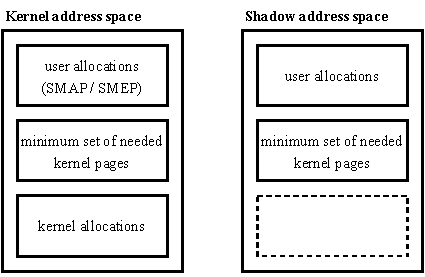
\includegraphics[page=1,width=.4\textwidth]{fig/prebuilt_shadow_address_space}
  \end{center}
  \caption{Kernel and shadow address space}
  \label{fig:shadow_address_space}
\end{figure}

Whenever a system call occurs in user mode the address space is switched from the shadow address space to the kernel address space.
As each core has its own \code{CR3}-register (the entrypoint to the currently active page table) no two threads can be executed at the same time and inadvertendly change one anothers address space.
The page table structure is not modified as the whole table is switched to a different one, thus not requiring synchronization between threads.
Thus this behaviour solves the multithreading challenge as no two threads can be executed on the same core at the same time with one being in kernel mode while the other is not, which would lead to the same address space being used by both allowing for microarchitectural flaws to be exploited or requiring synchronization for page table structures.

To implement switching between the address spaces with as little overhead as possible there needs to be a way to distinguish between them and get the address of the respective other address space using only the \code{CR3}-register and very little computation.
This is done by enforcing a strict placement of the PML4 page table, which is the top-most and thus entrypoint to the page table hierarchy, such that a single bit encodes the address space in use.
The 12th bit in the address is chosen for this purpose.
A \code{0} refers to the kernel address space and a \code{1} to the shadow address space (\autoref{fig:cr3-register}).
Simple bit manipulation allows computing the address of the other address space and determining which address space is active.

\begin{figure}[h]
  \begin{center}
    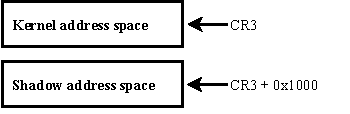
\includegraphics[page=1,width=.35\textwidth]{fig/prebuilt_cr3-register}
  \end{center}
  \caption{Behaviour of the CR3 register}
  \label{fig:cr3-register}
\end{figure}

Memory overhead introduced by the above is small: 8KB per thread, 12KB per process and 1 MB globally in the kernel.\cite{kaiser}

Quite a few pages are required to be mapped in both address spaces, unless a significant amount of reworking is done.
The mapped pages include:

\begin{itemize}
  \item{\textit{Interrupt Descriptor Table} (IDT) and interrupt entry and exit \code{.text} sections,}
  \item{entire per-CPU memory sections including \textit{Interrupt Request Stack and Vector} (IRQ), \textit{Task State Segment} (TSS) and \textit{Global Descriptor Table} (GDT),}
  \item{thread stacks as the CPU pushes registers on the current kernel stack which can either be a thread stack or an already saved per-CPU stack.}
\end{itemize}

x86 CPUs have the concept of global bits which indicate that a page mapping is global to every address space and thus does not need to be flushed with the rest of the TLB when switching address spaces.
This however exposes these pages to side-channel attacks as they are the same kernel pages that were meant to be hidden from shadow address spaces.
The Linux kernel uses global bits quite extensively to reduce the impact of TLB flushes as less pages are affected by a flush.
Disabling global bits did however not incur a significant performance penalty as the evaluation of \textit{D. Gruss et al.} \cite{kaiser} shows.
They suggest that CPUs likely already implement mechanisms to reduce the impact of TLB flushes such as tagging entries with their corresponding \code{CR3}-register values and not flushing entries for frequently used \code{CR3}-register values.
This behaviour was first described by \textit{Venkatasubramanian et al.} \cite{tlb-management-framework}.
In the end the performance impact of disabling global bits were negligible according to the testing of \textit{D. Gruss et al.} \cite{kaiser}.

Thus all three challenges can be solved by this approach.
